% A ieeeaccess.cls redefines \year as a macro (\year{...} sets the footer year). pgf/TikZ reads
% \year to seed random numbers and breaks with "Missing number". Keep the primitive and lend it to TikZ.
\let\TeXyear\year
\documentclass{ieeeaccess}

% ---- Encoding and language ----
\usepackage[utf8]{inputenc}
\usepackage[T1]{fontenc}
\usepackage[english]{babel}

% ---- Packages ----
\usepackage{cite}
\usepackage{amsmath,amssymb,amsfonts}
\usepackage{graphicx}
\usepackage{textcomp}
\usepackage{url}
\let\IEEEyear\year\let\year\TeXyear
\usepackage{tikz}
\let\year\IEEEyear
\usetikzlibrary{arrows.meta,positioning,fit,backgrounds,shapes.geometric}
\usepackage{array}
\usepackage{booktabs}
\usepackage{placeins}
\usepackage{etoolbox}
\newcolumntype{L}[1]{>{\raggedright\arraybackslash}p{#1}}
\makeatletter\g@addto@macro{\UrlBreaks}{\do\-\do\_}\makeatother
\extrafloats{100}

% ---- Compatibility with the IEEE Access class (see the course version for the reasons) ----
\definecolor{accessblue}{RGB}{0,86,155}
\definecolor{greycolor}{RGB}{51,51,51}
\makeatletter
\gdef\xfigwd{0pt}
\def\semvolume#1{\patchcmd{#1}{VOLUME\ \thevol, 2016}{}{}{%
  \patchcmd{#1}{VOLUME\ \thevol, \theyear}{}{}{\errmessage{footer: pattern not found}}}}
\semvolume\ps@headings\semvolume\ps@headings
\semvolume\ps@titlepage\semvolume\ps@titlepage
\pagestyle{headings}
\makeatother

% Pending marker: anything in red still needs a number from the bench or a decision. Remove before submission.
\newcommand{\pendente}[1]{\textcolor{red}{[PENDING: #1]}}

\begin{document}
\history{Research article prepared from the EC343E course project (UNIFEI, 2026). Bench data and code: https://github.com/ricardomdcj/cybersec-pkes-relay.}
\doi{}

\title{Relay Attacks on BLE Digital Keys: Measuring the Latency Budget of Challenge--Response Authentication}

\author{\uppercase{Ricardo Magno do Carmo J\'unior}\authorrefmark{1} AND \uppercase{Johny Francisco da Silva}\authorrefmark{1}}
\address[1]{Graduate Program in Electrical Engineering (PPG-EEL), Universidade Federal de Itajub\'a (UNIFEI), Itajub\'a, MG, Brazil (e-mail: ricardomdcj@gmail.com; johnyfsilva@gmail.com)}

\markboth
{do Carmo J\'unior and da Silva: Relay Attacks on BLE Digital Keys}
{do Carmo J\'unior and da Silva: Relay Attacks on BLE Digital Keys}

\begin{abstract}
Passive keyless entry systems infer proximity from radio range instead of measuring distance, and a relay attack defeats them by extending the radio channel without breaking any cryptography. Digital keys based on Bluetooth Low Energy (BLE) inherit the same assumption. We built a four-board bench with four ESP32-2432S028R (CYD) boards, acting as the key emulator, the verifier (vehicle), and two relays that carry a nonce-based HMAC challenge--response over the GATT layer through an ESP-NOW tunnel. Across 117 valid campaigns at 0.52, 0.99 and 2.24\,m, a relayed round added a median of about 280\,ms to the honest round-trip time (campaign-level 95\,\% interval 263 to 297\,ms at 2.24\,m, 28 campaigns per side). Every unicast relayed round was answered within the verifier's 2\,s timeout. When we injected a fixed delay in Relay B, the relay stopped authenticating once the delay exceeded about 1,650\,ms (the 50\,\% point lies between 1,640 and 1,675\,ms), which matches the timeout minus the honest relayed round-trip time of 1,641\,ms. A latency bound of 160\,ms, fixed before a replication set of ten direct and ten relayed campaigns, rejected no honest round in 500 and accepted 2.6\,\% of relayed rounds. Honest and relayed round-trip times overlap between about 107 and 150\,ms, so no single bound separates them completely. Between 0.52 and 2.24\,m the round-trip overhead showed no trend across 0.52, 0.99 and 2.24\,m, with ten campaigns per side at each, and RSSI separated the two configurations only through the physical layout. The verifier's timeout therefore sets the relay's latency budget, and a bound on round-trip time trades honest rejections against relayed acceptances rather than removing the relay.
\end{abstract}

\begin{keywords}
Bluetooth Low Energy, digital key, distance bounding, ESP32, latency, passive keyless entry, relay attack.
\end{keywords}

\titlepgskip=-15pt

\maketitle

\section{Introduction}
\label{sec:introduction}

\PARstart{V}{ehicles} with passive keyless entry and start (PKES) unlock the doors and authorize the engine start when the key is near, without any action by the driver. The convenience rests on an implicit safety premise: if the key answers the vehicle, the key is nearby. A relay attack breaks that premise. Two attackers extend the short-range channel between the vehicle and the key, so the key answers as if it were beside the car, and no secret is recovered or cloned~\cite{b1}.

Digital keys based on BLE, the phone-as-a-key model, use the same inference. They replace the low-frequency and UHF pair with a radio that the phone already carries, and the Car Connectivity Consortium specifies them~\cite{b9}. Relay attacks against BLE keys have been demonstrated~\cite{b3,b4}. These reports establish feasibility. They do not measure how the added latency, the distance and the verifier's decision interact on the same bench, with a control condition without relay.

This paper provides that measurement. We built a bench of four identical CYD boards: a key emulator, a verifier that plays the vehicle, and two relays. The relays tunnel the GATT challenge and response over ESP-NOW. The verifier records the round-trip time of every round, with and without the relay, and the decision it takes. We ask two research questions. RQ1: what overhead and success rate does a BLE relay add relative to a direct connection? RQ2: at which latency, and at which distance, does the relay stop authenticating? A third question, RQ3, asks whether round-trip time or RSSI discriminates a legitimate key from a relay.

The contributions are three. (i) A reproducible protocol and a measurement bench for a BLE challenge--response with and without relay, released with firmware, scripts, raw logs and hashes. (ii) A dataset of 117 campaigns, each with 50 rounds, and the campaign-level statistics that the dataset supports. (iii) An empirical characterization of the relay's latency budget: a timing bound that separates the two configurations on this stack, a latency sweep that locates the failure point, and an analysis of which signals discriminate. The results show that the verifier's timeout is the quantity that limits the relay, and that a round-trip-time bound is a trade-off, not a complete defence.

Section~\ref{sec:background} places the work against the related literature. Section~\ref{sec:threat} states the threat model and the scope. Section~\ref{sec:bench} describes the bench and the measurement protocol. Section~\ref{sec:method} gives the design and the statistics. Section~\ref{sec:results} reports the results, Section~\ref{sec:discussion} discusses the mitigations against the measured data, Section~\ref{sec:threats} lists the threats to validity, and Section~\ref{sec:conclusion} concludes.

\section{Background and Related Work}
\label{sec:background}

\subsection{Proximity inference and the relay}

PKES systems use a low-frequency (LF) wake-up signal of about 125 to 135\,kHz, whose range is a few metres, and an UHF response at 315 or 433\,MHz with a much longer range. A relay captures the wake-up near the car and re-emits it near the key, while the key's UHF response travels back unchanged. Francillon \emph{et al.} measured, for ten car models, the spread of the key's response time, which ranged from 11 to 436\,$\mu$s, and the maximum delay each car accepted, which ranged from 35\,$\mu$s to tens of milliseconds. Their wireless relay added about 120\,ns in one direction over 30\,m~\cite{b1}. Because the spread of the key's own response time is far larger than the delay a relay adds, timing alone was not a reliable detector in that work.

\subsection{Relays against BLE digital keys}

Staat \emph{et al.} built an analog physical-layer relay from off-the-shelf radio parts. In their cable-based proof of concept, the relay unlocked a car and a smart lock and started the engine while the legitimate smartphone was more than 65\,m away~\cite{b3}. Khan's advisory describes a relay at the BLE link layer against a Tesla Model~3 (2020). The relay added as little as 8\,ms of round-trip latency and stayed effective with up to 80\,ms of added round-trip latency, with the phone about 25\,m away~\cite{b4}. Xie \emph{et al.} analysed the Phone Key of a Tesla Model~3 and demonstrated a man-in-the-middle attack against it~\cite{b25}. None of these studies controls the added latency, and none reports a control condition without relay on the same bench.

\subsection{Distance bounding and ranging}

Distance-bounding protocols time a short challenge--response exchange, so that a relay that adds delay can only increase the distance estimate~\cite{b16,b27,b28}. Their security depends on the time resolution of the device: a relay adds propagation and processing time, and the bound is only as tight as the clock. Ultra-wideband (UWB) ranging offers that resolution, and the IEEE 802.15.4z amendment defines its secure form~\cite{b30}. Several works show that the secure ranging can still be attacked: Singh \emph{et al.} analysed the HRP time-of-flight measurement~\cite{b6}, Leu \emph{et al.} reduced the measured distance with ghost peaks~\cite{b7}, and Anliker \emph{et al.} broke secure ranging through the clock~\cite{b8}. Singh \emph{et al.} also proposed pulse reordering as a defence~\cite{b5}. A BLE radio that is not designed for ranging offers a coarser clock, which is the constraint this bench works under.

\subsection{Detectors and the gap}

Wang, Lounis and Zulkernine combined RSSI, round-trip time and other context to detect relays against a dedicated key~\cite{b22}, and Revadigar \emph{et al.} used BLE RSSI and user activity to decide proximity for a smartphone key~\cite{b23}. Abidin \emph{et al.} implemented narrow-band ranging with time of flight on a dedicated chip~\cite{b24}, Suresh \emph{et al.} combined BLE, UWB and NFC for a vehicle access prototype~\cite{b10}, and a later work uses BLE channel sounding for ranging~\cite{b26}. The detectors in this group measure the accuracy of a classifier or of a ranging method. They do not measure how a relay changes the authentication decision of an unmodified protocol, as a function of latency and distance, with a repeated control condition. That measurement is the gap this paper addresses.

\section{Threat Model and Scope}
\label{sec:threat}

The attacker places Relay~A next to the key and Relay~B next to the vehicle. Relay~A acts as a BLE central towards the key, and Relay~B acts as a BLE peripheral towards the verifier. The two relays exchange the challenge and the response over ESP-NOW. Each relay sees the GATT values in transit, but neither knows the pre-shared secret, and neither can produce a valid response. The attacker cannot break the HMAC, clone the key, or replay an old response, because every challenge is a fresh 16-byte nonce. The relay is therefore a live forwarder that exploits the proximity inference, not a cryptographic attack.

The scope is deliberately narrow. The object is a BLE challenge--response over GATT with a pre-shared key, emulated by ESP32 boards. The study does not test a smartphone key, a real vehicle, the PKES LF/UHF system, or any product. It does not test the 2\,Mbit/s or Coded PHYs, because the ESP32 is a BLE~4.2 device that supports only the 1\,Mbit/s PHY. All experiments run on boards owned by the authors, in a closed bench. A stop rule ends any test that could interfere with third-party devices in the 2.4\,GHz band.

\section{Bench and Measurement Protocol}
\label{sec:bench}

\subsection{Architecture}

Fig.~\ref{fig:architecture} shows the four boards. The key emulator runs the key firmware, a GATT server with the same service, characteristics and HMAC as the contract. The verifier runs the vehicle firmware, a BLE central that writes a nonce, waits for the notification, and decides: it authenticates a round only if the HMAC matches and the response arrives within 2\,s. The two relays run one firmware image in two roles.

\begin{figure*}[t]
\centering
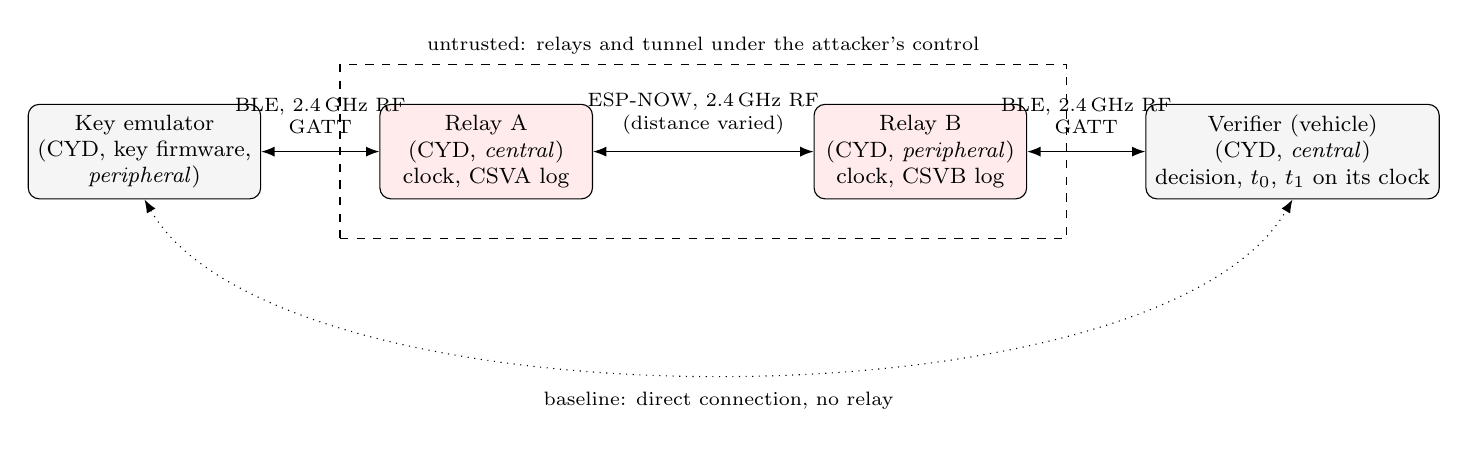
\begin{tikzpicture}[
  node distance=8mm and 15mm,
  box/.style={draw, rounded corners, align=center, font=\footnotesize, minimum height=12mm, minimum width=27mm, fill=gray!8},
  atk/.style={box, fill=red!8},
  lbl/.style={font=\scriptsize, align=center},
  boundary/.style={draw, dashed, inner sep=5mm},
  >=Latex
]
\node[box] (key) {Key emulator\\(CYD, key firmware,\\\emph{peripheral})};
\node[atk, right=of key] (relA) {Relay A\\(CYD, \emph{central})\\clock, CSVA log};
\node[atk, right=28mm of relA] (relB) {Relay B\\(CYD, \emph{peripheral})\\clock, CSVB log};
\node[box, right=of relB] (veh) {Verifier (vehicle)\\(CYD, \emph{central})\\decision, $t_0$, $t_1$ on its clock};
\draw[<->] (key) -- (relA) node[midway, above=1mm, lbl]{BLE, 2.4\,GHz RF\\GATT};
\draw[<->] (relA) -- (relB) node[midway, above=1mm, lbl]{ESP-NOW, 2.4\,GHz RF\\(distance varied)};
\draw[<->] (relB) -- (veh) node[midway, above=1mm, lbl]{BLE, 2.4\,GHz RF\\GATT};
\node[boundary, fit=(relA)(relB), label={[font=\scriptsize]above:untrusted: relays and tunnel under the attacker's control}] (boundaryNode) {};
\draw[<->, dotted] (key.south) to[out=-60,in=-120,looseness=0.6] node[pos=0.5, below=1mm, lbl]{baseline: direct connection, no relay} (veh.south);
\end{tikzpicture}
\caption{Bench architecture. Four ESP32-2432S028R (CYD) boards: the key emulator, Relay~A next to it, Relay~B next to the verifier, and the verifier. The two relays and the ESP-NOW tunnel between them form the untrusted region (dashed). Every link is bidirectional: the challenge goes from the verifier to the key and the response comes back the same way. The authentication decision and the timestamps $t_0$ and $t_1$ stay in the verifier. In the baseline the key connects directly to the verifier (dotted). Clocks: each board's esp\_timer (1\,$\mu$s resolution); the verifier stamps $t_0$ at the challenge write and $t_1$ at the notification, and the relays log their turnarounds (CSVA, CSVB). The three solid links are 2.4\,GHz RF hops; the dashed boundary is the attacker's region.}
\label{fig:architecture}
\end{figure*}

\subsection{Hardware and firmware}

All four boards are ESP32-2432S028R (CYD) modules: a classic ESP32 with BLE~4.2 and a 1\,Mbit/s PHY, a 320$\times$240 display and an RGB LED. The firmware is written for ESP-IDF v6.1 with the NimBLE host, and the user interface uses LVGL~8.3. The contract fixes the service UUID \texttt{8f2a0001-1b2c-4e6a-9f3d-2a7c1e5b0a10}, a CHALLENGE characteristic (write), and a RESPONSE characteristic (notify). The nonce has 16 bytes, the response is HMAC-SHA256 truncated to 16 bytes, and the pre-shared key is a bench constant in the source, so an attacker who reads the source can compute valid responses. This does not affect the relay, which never needs the key.

The verifier measures the round trip with \texttt{esp\_timer} (1\,$\mu$s resolution) between the write of the challenge and the arrival of the notification. The connection interval is negotiated to 50\,ms, the MTU to 256 bytes, and the round grid to one round per second. Since 1\,s is a multiple of 50\,ms, every round of a campaign keeps the same phase of the connection grid. From the M-19 firmware onward, each campaign starts at a random offset within one period, so the campaigns sample different phases. The verifier's timeout is 2\,s. A response that arrives after its round has timed out is recognised by its nonce and discarded (M-22). Before that change, such a response was taken for the answer to the round in flight; no late response occurs in the campaigns recorded before the change.

Relay~B has one bench command beyond the transmit power: \texttt{DELAY} $D$ holds every vehicle challenge for $D$\,ms before it goes on the tunnel, using a timer so that the BLE host task is not blocked. The command is used only for the latency sweep, and it is off by default.

\subsection{Layouts and distances}

The distances are the layout on the bench, estimated by the operator and not measured with an instrument. We used three layouts. At 0.52\,m the relays were placed between the car and the key, and their exact positions were not recorded. At 0.99\,m the car and Relay~B were 12\,cm apart, Relay~A and the key 12\,cm apart, and the two relays 75\,cm apart, so the car-to-key distance is about 0.99\,m. At 2.24\,m the same 12\,cm offsets surrounded relays 2\,m apart. The campaigns before the M-19 firmware were recorded at 0.52, 0.99 and 2.24\,m, and the campaigns with the M-19 firmware at 2.24\,m and at 0.99\,m.

\subsection{Campaign procedure}

A campaign is 50 rounds. The campaign scripts in \texttt{tools/campaign} open the four serial consoles, start the campaign and log every port.The campaign label and the distance are written to the verifier's log, and the injected delay is logged by Relay~B. Every campaign keeps its capture and a manifest with the firmware commit, and every aborted or invalid session is kept in a separate folder with its reason. The order of the campaigns alternated between baseline and relayed, and was not randomized. We report this as a limitation in Section~\ref{sec:threats}.

\section{Methodology}
\label{sec:method}

\subsection{Research questions and hypotheses}

RQ1 asks for the overhead and success of the relay. RQ2 asks at which distance and latency the relay stops authenticating. RQ3 asks which signal, round-trip time or RSSI, discriminates a legitimate key from a relay. We test three hypotheses. H1: latency is the main discriminant, supported if the relayed round-trip distribution separates from the baseline with a large effect size and the baseline variation is small compared with the overhead. H2: the authentication failures come from the implementation and the timeout more than from the distance, supported if the success rate follows the timeout and not the distance. H3: RSSI adds no stable discrimination once the environment and power are controlled, supported if RSSI does not separate the configurations for a reason unrelated to the relay.

\subsection{Unit of analysis and statistics}

The unit of inference is the campaign. Rounds inside a campaign share one phase of the connection grid, so round-level p-values would be pseudo-replicated. We therefore test campaign medians with the Mann--Whitney test, exact for the small sets and normal-approximated otherwise, and report the effect size as Cliff's $\delta=2\,\mathrm{AUC}-1$. Confidence intervals come from a cluster bootstrap that resamples campaigns within each condition, with 2000 resamples and a fixed seed. Proportions have Wilson intervals. The campaign-level p-values of the eight groups in Table~\ref{tab:overhead} are corrected with Holm's method. Round-level values are reported as descriptive only. We did not fit a logistic or a mixed model; the campaign-level tests and the cluster bootstrap are the approximations used instead.

For the sample size, we used the effect that matters for the design. We take $\Delta=25$\,ms, half the BLE connection interval, as the smallest difference of interest. The required number of campaigns per group is $n = 2(z_{0.975}+z_{0.80})^2\sigma^2/\Delta^2$, with $\sigma$ the campaign-to-campaign standard deviation of the medians.

\subsection{Experiments}

E1 measures the overhead at each layout. E2 injects a delay of 0 to 2.2\,s into Relay~B at 0.99\,m, and measures the success rate of the relayed rounds. E3 applies a fixed bound $T$ to the round-trip time and measures the honest rounds rejected and the relayed rounds accepted. The bound was first read from one set of campaigns, then tested on a held-out set, and then replicated on a set whose criteria were fixed before its campaigns were recorded (the plans are committed in the repository before the data). E4 compares the round-trip time and RSSI of the two configurations. E5 counts the timeouts of each transport.

\section{Results}
\label{sec:results}

\subsection{Overhead and campaign-level statistics}

At 2.24\,m every relayed unicast round was answered and authenticated: 1400 rounds in the three sets with the M-19 firmware, and 300 more in the earlier sets. Table~\ref{tab:overhead} gives the medians and the overhead, with the campaign-level bootstrap intervals. Across the 28 direct and 28 relayed campaigns at 2.24\,m the median round trip was 79.1\,ms without the relay and 358.5\,ms with it, an overhead of 279.5\,ms (95\,\% interval 262.5 to 296.6\,ms). The campaign medians of the two configurations separate completely (Cliff's $\delta=1.00$, exact Mann--Whitney $p\le 0.0002$ in each set, Holm-adjusted $p\le0.0006$). The three independent sets measured the overhead at 323\,ms (in sample), 276\,ms (held-out) and 275\,ms (replication).

\begin{table*}[t]
\caption{Overhead of the relayed unicast configuration over the direct baseline, campaign level. Medians of the answered rounds; intervals are 95\,\% cluster bootstrap over campaigns.}
\label{tab:overhead}
\centering
\footnotesize
\begin{tabular}{L{3.9cm}L{2.2cm}L{2.2cm}L{2.2cm}L{3.9cm}}
\toprule
\textbf{Set} & \textbf{Campaigns (direct, relayed)} & \textbf{Median direct (ms)} & \textbf{Median relayed (ms)} & \textbf{Overhead (ms), 95\,\% CI} \\
\midrule
2.24\,m, M-19, in sample & 8, 8 & 74.7 & 397.5 & 322.8 (273.9 to 343.8) \\
2.24\,m, held-out & 10, 10 & 81.2 & 356.7 & 275.5 (211.5 to 297.4) \\
2.24\,m, replication & 10, 10 & 80.2 & 354.7 & 274.6 (225.7 to 305.4) \\
2.24\,m, all M-19 & 28, 28 & 79.1 & 358.5 & 279.5 (262.5 to 296.6) \\
0.99\,m, M-19 & 10, 10 & 90.4 & 379.6 & 289.2 (246.9 to 301.7) \\
0.52\,m, M-19 & 10, 10 & 90.0 & 371.5 & 281.5 (248.2 to 309.6) \\
\midrule
0.52\,m, earlier firmware & 3, 3 & 76.9 & 384.6 & 307.7 (215.1 to 319.6) \\
0.99\,m, earlier firmware & 3, 3 & 82.0 & 376.6 & 294.6 (273.4 to 340.0) \\
2.24\,m, earlier firmware & 3, 3 & 85.7 & 364.5 & 278.9 (274.8 to 366.8) \\
\bottomrule
\end{tabular}
\end{table*}

Fig.~\ref{fig:overhead} shows every campaign median, so the spread between campaigns is visible next to the overhead.

\begin{figure*}[t]
\centering
% Campaign medians (dots) and the median of each configuration (bar). Generated by tools/make_paper_figures.py.
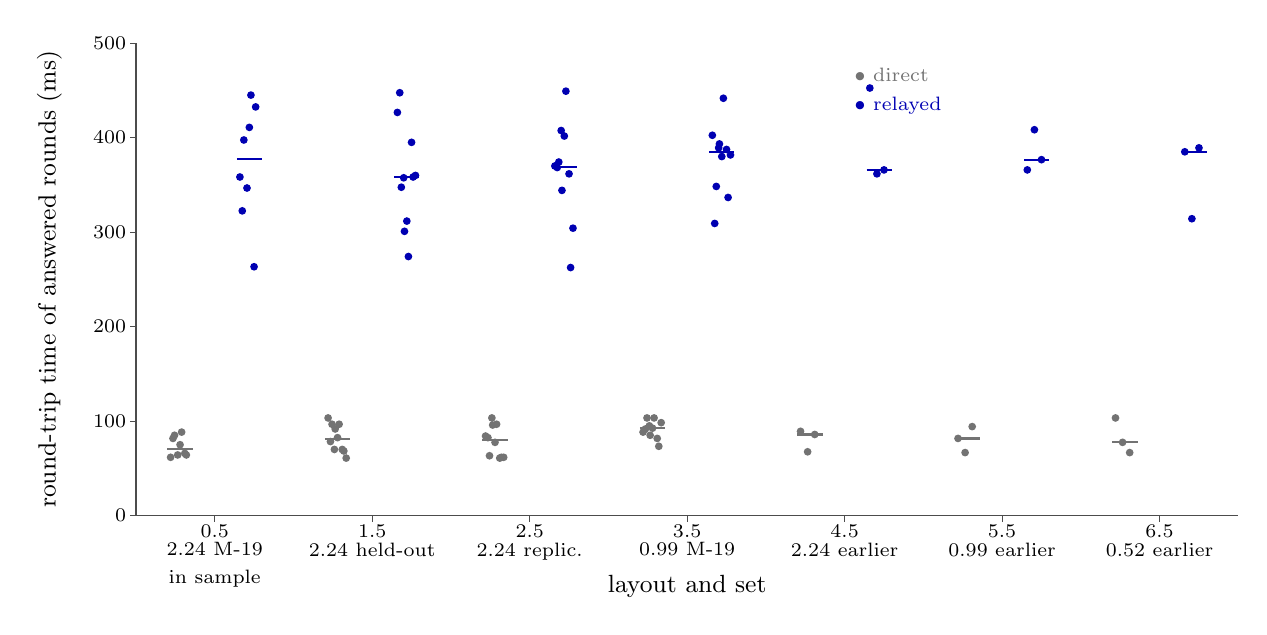
\begin{tikzpicture}[>=Latex, font=\footnotesize]
\draw[black!70] (0,0) -- (14,0);
\draw[black!70] (0,0) -- (0,6);
\draw[black!70] (1,0) -- ++(0,-0.08);
\node[font=\scriptsize, below] at (1,0) {0.5};
\draw[black!70] (3,0) -- ++(0,-0.08);
\node[font=\scriptsize, below] at (3,0) {1.5};
\draw[black!70] (5,0) -- ++(0,-0.08);
\node[font=\scriptsize, below] at (5,0) {2.5};
\draw[black!70] (7,0) -- ++(0,-0.08);
\node[font=\scriptsize, below] at (7,0) {3.5};
\draw[black!70] (9,0) -- ++(0,-0.08);
\node[font=\scriptsize, below] at (9,0) {4.5};
\draw[black!70] (11,0) -- ++(0,-0.08);
\node[font=\scriptsize, below] at (11,0) {5.5};
\draw[black!70] (13,0) -- ++(0,-0.08);
\node[font=\scriptsize, below] at (13,0) {6.5};
\draw[black!70] (0,0) -- ++(-0.08,0);
\node[font=\scriptsize, left] at (0,0) {0};
\draw[black!70] (0,1.2) -- ++(-0.08,0);
\node[font=\scriptsize, left] at (0,1.2) {100};
\draw[black!70] (0,2.4) -- ++(-0.08,0);
\node[font=\scriptsize, left] at (0,2.4) {200};
\draw[black!70] (0,3.6) -- ++(-0.08,0);
\node[font=\scriptsize, left] at (0,3.6) {300};
\draw[black!70] (0,4.8) -- ++(-0.08,0);
\node[font=\scriptsize, left] at (0,4.8) {400};
\draw[black!70] (0,6) -- ++(-0.08,0);
\node[font=\scriptsize, left] at (0,6) {500};
\node[font=\small] at (7,-0.9) {layout and set};
\node[font=\small, rotate=90] at (-1.1,3) {round-trip time of answered rounds (ms)};
\node[font=\scriptsize, below] at (1,-0.22) {2.24 M-19};
\node[font=\scriptsize, below] at (1,-0.57) {in sample};
\fill[black!55] (0.44,0.74) circle (1.4pt);
\fill[black!55] (0.53,0.77) circle (1.4pt);
\fill[black!55] (0.62,0.79) circle (1.4pt);
\fill[black!55] (0.47,0.98) circle (1.4pt);
\fill[black!55] (0.56,0.9) circle (1.4pt);
\fill[black!55] (0.64,0.77) circle (1.4pt);
\fill[black!55] (0.49,1.02) circle (1.4pt);
\fill[black!55] (0.58,1.06) circle (1.4pt);
\draw[black!55, thick] (0.4,0.85) -- (0.72,0.85);
\fill[blue!70!black] (1.32,4.3) circle (1.4pt);
\fill[blue!70!black] (1.41,4.16) circle (1.4pt);
\fill[blue!70!black] (1.5,3.16) circle (1.4pt);
\fill[blue!70!black] (1.35,3.87) circle (1.4pt);
\fill[blue!70!black] (1.44,4.93) circle (1.4pt);
\fill[blue!70!black] (1.52,5.19) circle (1.4pt);
\fill[blue!70!black] (1.37,4.77) circle (1.4pt);
\fill[blue!70!black] (1.46,5.34) circle (1.4pt);
\draw[blue!70!black, thick] (1.28,4.53) -- (1.6,4.53);
\node[font=\scriptsize, below] at (3,-0.22) {2.24 held-out};
\fill[black!55] (2.44,1.24) circle (1.4pt);
\fill[black!55] (2.53,1.1) circle (1.4pt);
\fill[black!55] (2.62,0.84) circle (1.4pt);
\fill[black!55] (2.47,0.94) circle (1.4pt);
\fill[black!55] (2.56,0.99) circle (1.4pt);
\fill[black!55] (2.64,0.82) circle (1.4pt);
\fill[black!55] (2.49,1.16) circle (1.4pt);
\fill[black!55] (2.58,1.16) circle (1.4pt);
\fill[black!55] (2.67,0.73) circle (1.4pt);
\fill[black!55] (2.52,0.84) circle (1.4pt);
\draw[black!55, thick] (2.4,0.97) -- (2.72,0.97);
\fill[blue!70!black] (3.32,5.12) circle (1.4pt);
\fill[blue!70!black] (3.41,3.61) circle (1.4pt);
\fill[blue!70!black] (3.5,4.74) circle (1.4pt);
\fill[blue!70!black] (3.35,5.37) circle (1.4pt);
\fill[blue!70!black] (3.44,3.74) circle (1.4pt);
\fill[blue!70!black] (3.52,4.3) circle (1.4pt);
\fill[blue!70!black] (3.37,4.17) circle (1.4pt);
\fill[blue!70!black] (3.46,3.29) circle (1.4pt);
\fill[blue!70!black] (3.55,4.32) circle (1.4pt);
\fill[blue!70!black] (3.4,4.29) circle (1.4pt);
\draw[blue!70!black, thick] (3.28,4.3) -- (3.6,4.3);
\node[font=\scriptsize, below] at (5,-0.22) {2.24 replic.};
\fill[black!55] (4.44,1.01) circle (1.4pt);
\fill[black!55] (4.53,1.15) circle (1.4pt);
\fill[black!55] (4.62,0.73) circle (1.4pt);
\fill[black!55] (4.47,0.99) circle (1.4pt);
\fill[black!55] (4.56,0.93) circle (1.4pt);
\fill[black!55] (4.64,0.74) circle (1.4pt);
\fill[black!55] (4.49,0.76) circle (1.4pt);
\fill[black!55] (4.58,1.16) circle (1.4pt);
\fill[black!55] (4.67,0.74) circle (1.4pt);
\fill[black!55] (4.52,1.24) circle (1.4pt);
\draw[black!55, thick] (4.4,0.96) -- (4.72,0.96);
\fill[blue!70!black] (5.32,4.44) circle (1.4pt);
\fill[blue!70!black] (5.41,4.13) circle (1.4pt);
\fill[blue!70!black] (5.5,4.34) circle (1.4pt);
\fill[blue!70!black] (5.35,4.42) circle (1.4pt);
\fill[blue!70!black] (5.44,4.82) circle (1.4pt);
\fill[blue!70!black] (5.52,3.15) circle (1.4pt);
\fill[blue!70!black] (5.37,4.49) circle (1.4pt);
\fill[blue!70!black] (5.46,5.39) circle (1.4pt);
\fill[blue!70!black] (5.55,3.65) circle (1.4pt);
\fill[blue!70!black] (5.4,4.89) circle (1.4pt);
\draw[blue!70!black, thick] (5.28,4.43) -- (5.6,4.43);
\node[font=\scriptsize, below] at (7,-0.22) {0.99 M-19};
\fill[black!55] (6.44,1.06) circle (1.4pt);
\fill[black!55] (6.53,1.02) circle (1.4pt);
\fill[black!55] (6.62,0.98) circle (1.4pt);
\fill[black!55] (6.47,1.1) circle (1.4pt);
\fill[black!55] (6.56,1.11) circle (1.4pt);
\fill[black!55] (6.64,0.88) circle (1.4pt);
\fill[black!55] (6.49,1.24) circle (1.4pt);
\fill[black!55] (6.58,1.24) circle (1.4pt);
\fill[black!55] (6.67,1.18) circle (1.4pt);
\fill[black!55] (6.52,1.14) circle (1.4pt);
\draw[black!55, thick] (6.4,1.11) -- (6.72,1.11);
\fill[blue!70!black] (7.32,4.83) circle (1.4pt);
\fill[blue!70!black] (7.41,4.72) circle (1.4pt);
\fill[blue!70!black] (7.5,4.65) circle (1.4pt);
\fill[blue!70!black] (7.35,3.71) circle (1.4pt);
\fill[blue!70!black] (7.44,4.56) circle (1.4pt);
\fill[blue!70!black] (7.52,4.04) circle (1.4pt);
\fill[blue!70!black] (7.37,4.18) circle (1.4pt);
\fill[blue!70!black] (7.46,5.3) circle (1.4pt);
\fill[blue!70!black] (7.55,4.58) circle (1.4pt);
\fill[blue!70!black] (7.4,4.67) circle (1.4pt);
\draw[blue!70!black, thick] (7.28,4.62) -- (7.6,4.62);
\node[font=\scriptsize, below] at (9,-0.22) {2.24 earlier};
\fill[black!55] (8.44,1.07) circle (1.4pt);
\fill[black!55] (8.53,0.81) circle (1.4pt);
\fill[black!55] (8.62,1.03) circle (1.4pt);
\draw[black!55, thick] (8.4,1.03) -- (8.72,1.03);
\fill[blue!70!black] (9.32,5.43) circle (1.4pt);
\fill[blue!70!black] (9.41,4.34) circle (1.4pt);
\fill[blue!70!black] (9.5,4.39) circle (1.4pt);
\draw[blue!70!black, thick] (9.28,4.39) -- (9.6,4.39);
\node[font=\scriptsize, below] at (11,-0.22) {0.99 earlier};
\fill[black!55] (10.44,0.98) circle (1.4pt);
\fill[black!55] (10.53,0.8) circle (1.4pt);
\fill[black!55] (10.62,1.13) circle (1.4pt);
\draw[black!55, thick] (10.4,0.98) -- (10.72,0.98);
\fill[blue!70!black] (11.32,4.39) circle (1.4pt);
\fill[blue!70!black] (11.41,4.9) circle (1.4pt);
\fill[blue!70!black] (11.5,4.52) circle (1.4pt);
\draw[blue!70!black, thick] (11.28,4.52) -- (11.6,4.52);
\node[font=\scriptsize, below] at (13,-0.22) {0.52 earlier};
\fill[black!55] (12.44,1.24) circle (1.4pt);
\fill[black!55] (12.53,0.93) circle (1.4pt);
\fill[black!55] (12.62,0.8) circle (1.4pt);
\draw[black!55, thick] (12.4,0.93) -- (12.72,0.93);
\fill[blue!70!black] (13.32,4.62) circle (1.4pt);
\fill[blue!70!black] (13.41,3.77) circle (1.4pt);
\fill[blue!70!black] (13.5,4.67) circle (1.4pt);
\draw[blue!70!black, thick] (13.28,4.62) -- (13.6,4.62);
\node[font=\scriptsize, anchor=west] at (9.0,5.6) {\textcolor{black!55}{$\bullet$ direct}};
\node[font=\scriptsize, anchor=west] at (9.0,5.2) {\textcolor{blue!70!black}{$\bullet$ relayed}};
\end{tikzpicture}

\caption{Campaign medians of the answered rounds for the direct baseline (grey) and the relayed unicast configuration (blue), per layout and set. The bar marks the median of each configuration. The spread between campaigns is the phase effect discussed in Section~\ref{sec:threats}.}
\label{fig:overhead}
\end{figure*}

The earlier sets, recorded before the start offset existed, have three campaigns per side. Their smallest possible two-sided exact p-value is 0.10, so they are descriptive. They show the same overhead of about 280 to 310\,ms at the three layouts, which is consistent with no distance dependence at the resolution of three campaigns per layout. The baseline spread is small: the interquartile range of the direct rounds is 20\,ms in the in-sample set and 29\,ms across all M-19 campaigns, against an overhead of about 280\,ms, so H1 is supported.

\subsection{Distance}

Between 0.52 and 2.24\,m the overhead stayed between about 275 and 310\,ms, and every unicast relayed round was answered. With the M-19 firmware and ten campaigns per side at each layout, the overhead is 282\,ms at 0.52\,m, 289\,ms at 0.99\,m and 280\,ms at 2.24\,m, with overlapping intervals (248 to 310, 247 to 302 and 263 to 297\,ms). Distance does not change the overhead beyond the campaign-to-campaign spread. The layouts differ in RSSI (Section~\ref{sec:rssi}), but RSSI does not follow one path-loss exponent across them. A link budget with the datasheet sensitivities puts the ESP-NOW tunnel range between about 50\,m and 2.3\,km at the default power, depending on the path-loss exponent. That is a model estimate, not a measurement, since the relays were never more than 2\,m apart. At 0.99\,m with the M-19 firmware (ten campaigns per side) the overhead was 289\,ms (95\,\% interval 247 to 302\,ms), against 280\,ms at 2.24\,m. The two intervals overlap, so the distance between 0.99 and 2.24\,m does not change the overhead beyond the campaign-to-campaign spread.

\subsection{The effectiveness limit: injected latency}
\label{sec:sweep}

Table~\ref{tab:sweep} and Fig.~\ref{fig:sweep} give the success of the relayed rounds at 0.99\,m as Relay~B adds a delay $D$ to each challenge. A round authenticates only if its response arrives within the 2\,s timeout. The relay works while $D$ plus the honest relayed round trip stays below the timeout, and fails after that. With the honest relayed median of 358.6\,ms at $D=0$, the expected threshold is 1,641\,ms, and the measured threshold, where success falls below 50\,\%, lies between 1,650 and 1,675\,ms (linear interpolation between the two campaigns that bracket 50\,\%: 1,656\,ms). Late answers do not decide the outcome. A late answer reaches the verifier only if relay~B has not yet received the next challenge; otherwise relay~B drops it (32 drops in the 1,750\,ms campaign). The verifier discards the late answers that do reach it (8, 22 and 36 in the 1,600, 1,650 and 1,700\,ms campaigns, M-22), and no sweep campaign contains a FAIL row.

\begin{table}[t]
\caption{Success of the relayed rounds at 0.99\,m versus the delay injected in Relay~B (one campaign of 50 rounds per delay). Wilson intervals at 95\,\%.}
\label{tab:sweep}
\centering
\footnotesize
\begin{tabular}{L{1.2cm}L{1.6cm}L{2.2cm}L{2.6cm}}
\toprule
\textbf{Delay (ms)} & \textbf{OK / rounds} & \textbf{Success (95\,\% CI)} & \textbf{Median RTT of OK rounds (ms)} \\
\midrule
0 & 50 / 50 & 100.0\,\% (92.9 to 100.0) & 358.6 \\
500 & 50 / 50 & 100.0\,\% (92.9 to 100.0) & 879.7 \\
1000 & 50 / 50 & 100.0\,\% (92.9 to 100.0) & 1382.3 \\
1400 & 50 / 50 & 100.0\,\% (92.9 to 100.0) & 1784.1 \\
1500 & 50 / 50 & 100.0\,\% (92.9 to 100.0) & 1784.9 \\
1600 & 36 / 50 & 72.0\,\% (58.3 to 82.5) & 1984.5 \\
1625 & 45 / 50 & 90.0\,\% (78.6 to 95.7) & 1980.3 \\
1650 & 27 / 50 & 54.0\,\% (40.4 to 67.0) & 1942.9 \\
1675 & 18 / 50 & 36.0\,\% (24.1 to 49.9) & 1884.1 \\
1700 & 8 / 50 & 16.0\,\% (8.3 to 28.5) & 1984.3 \\
1750 & 8 / 50 & 16.0\,\% (8.3 to 28.5) & 1965.0 \\
1800 & 0 / 50 & 0.0\,\% (0.0 to 7.1) & -- \\
1900 & 0 / 50 & 0.0\,\% (0.0 to 7.1) & -- \\
2200 & 0 / 50 & 0.0\,\% (0.0 to 7.1) & -- \\
\bottomrule
\end{tabular}
\end{table}

\begin{figure*}[t]
\centering
% Placeholder until the delay sweep is recorded; tools/make_paper_figures.py replaces it.
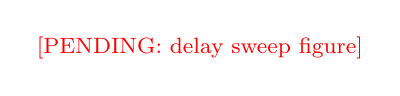
\begin{tikzpicture}[font=\footnotesize]
\node[red] at (3,1) {[PENDING: delay sweep figure]};
\end{tikzpicture}

\caption{Success of the relayed rounds at 0.99\,m versus the delay injected into Relay~B, one campaign per delay with 95\,\% Wilson intervals. The dashed line is 50\,\%. The relay stops authenticating when the injected delay plus the honest relayed round trip exceeds the 2\,s verifier timeout.}
\label{fig:sweep}
\end{figure*}

\subsection{Latency bound and its replication}
\label{sec:bound}

A bound $T$ on the round trip rejects an honest round when its RTT is above $T$ or when it gets no answer, and accepts a relayed round when it is answered within $T$. In the in-sample set of eight campaigns per side, the bound of 150\,ms rejected no honest round and accepted 1.5\,\% of relayed rounds. On a held-out set of ten campaigns per side, recorded after 150\,ms was fixed, one honest round in 500 took 150.6\,ms, so 150\,ms failed its no-false-reject criterion, while 160\,ms rejected none and accepted 1.4\,\% of relayed rounds. The 160\,ms value was chosen after that maximum was seen, so we replicated it on a new set of ten campaigns per side with the criteria fixed in advance. On the replication set, 160\,ms rejected 0 of 500 honest rounds (the largest honest RTT was 143.3\,ms) and accepted 13 of 500 relayed rounds (2.6\,\%; 95\,\% interval 1.5 to 4.4\,\%). Across the 28 direct and 28 relayed campaigns at 2.24\,m, 160\,ms rejected 0 of 1400 honest rounds and accepted 26 of 1400 relayed rounds (1.9\,\%). Fig.~\ref{fig:bound} shows the operating curve on the replication set.

\begin{figure*}[t]
\centering
% Operating curve of the 160 ms bound on the replication set (10 + 10 campaigns). Generated by tools/make_paper_figures.py.
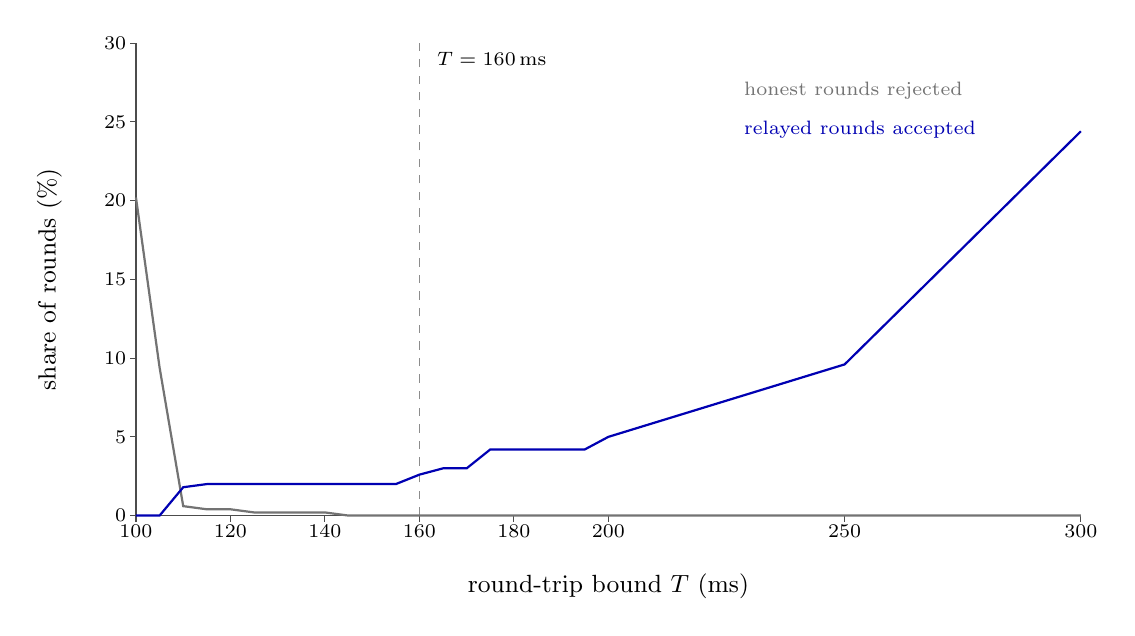
\begin{tikzpicture}[>=Latex, font=\footnotesize]
\draw[black!70] (0,0) -- (12,0);
\draw[black!70] (0,0) -- (0,6);
\draw[black!70] (0,0) -- ++(0,-0.08);
\node[font=\scriptsize, below] at (0,0) {100};
\draw[black!70] (1.2,0) -- ++(0,-0.08);
\node[font=\scriptsize, below] at (1.2,0) {120};
\draw[black!70] (2.4,0) -- ++(0,-0.08);
\node[font=\scriptsize, below] at (2.4,0) {140};
\draw[black!70] (3.6,0) -- ++(0,-0.08);
\node[font=\scriptsize, below] at (3.6,0) {160};
\draw[black!70] (4.8,0) -- ++(0,-0.08);
\node[font=\scriptsize, below] at (4.8,0) {180};
\draw[black!70] (6,0) -- ++(0,-0.08);
\node[font=\scriptsize, below] at (6,0) {200};
\draw[black!70] (9,0) -- ++(0,-0.08);
\node[font=\scriptsize, below] at (9,0) {250};
\draw[black!70] (12,0) -- ++(0,-0.08);
\node[font=\scriptsize, below] at (12,0) {300};
\draw[black!70] (0,0) -- ++(-0.08,0);
\node[font=\scriptsize, left] at (0,0) {0};
\draw[black!70] (0,1) -- ++(-0.08,0);
\node[font=\scriptsize, left] at (0,1) {5};
\draw[black!70] (0,2) -- ++(-0.08,0);
\node[font=\scriptsize, left] at (0,2) {10};
\draw[black!70] (0,3) -- ++(-0.08,0);
\node[font=\scriptsize, left] at (0,3) {15};
\draw[black!70] (0,4) -- ++(-0.08,0);
\node[font=\scriptsize, left] at (0,4) {20};
\draw[black!70] (0,5) -- ++(-0.08,0);
\node[font=\scriptsize, left] at (0,5) {25};
\draw[black!70] (0,6) -- ++(-0.08,0);
\node[font=\scriptsize, left] at (0,6) {30};
\node[font=\small] at (6,-0.9) {round-trip bound $T$ (ms)};
\node[font=\small, rotate=90] at (-1.1,3) {share of rounds (\%)};
\draw[black!45, dashed] (3.6,0) -- (3.6,6);
\node[font=\scriptsize, anchor=west] at (3.7,5.8) {$T=160$\,ms};
\draw[black!55, thick] (0,4.04) -- (0.3,1.88) -- (0.6,0.12) -- (0.9,0.08) -- (1.2,0.08) -- (1.5,0.04) -- (1.8,0.04) -- (2.1,0.04) -- (2.4,0.04) -- (2.7,0) -- (3,0) -- (3.3,0) -- (3.6,0) -- (3.9,0) -- (4.2,0) -- (4.5,0) -- (4.8,0) -- (5.1,0) -- (5.4,0) -- (5.7,0) -- (6,0) -- (9,0) -- (12,0);
\draw[blue!70!black, thick] (0,0) -- (0.3,0) -- (0.6,0.36) -- (0.9,0.4) -- (1.2,0.4) -- (1.5,0.4) -- (1.8,0.4) -- (2.1,0.4) -- (2.4,0.4) -- (2.7,0.4) -- (3,0.4) -- (3.3,0.4) -- (3.6,0.52) -- (3.9,0.6) -- (4.2,0.6) -- (4.5,0.84) -- (4.8,0.84) -- (5.1,0.84) -- (5.4,0.84) -- (5.7,0.84) -- (6,1) -- (9,1.92) -- (12,4.88);
\node[font=\scriptsize, anchor=west] at (7.6,5.4) {\textcolor{black!55}{honest rounds rejected}};
\node[font=\scriptsize, anchor=west] at (7.6,4.9) {\textcolor{blue!70!black}{relayed rounds accepted}};
\end{tikzpicture}

\caption{Operating curve of the round-trip bound on the replication set (ten direct and ten relayed campaigns, 2.24\,m). Honest rounds rejected (grey) and relayed rounds accepted (blue) as the bound $T$ varies. The dashed line marks the 160\,ms bound fixed before the replication campaigns.}
\label{fig:bound}
\end{figure*}

The relayed rounds that pass the bound come from a few campaigns: in each of the two sets, two relayed campaigns contributed every accepted round at 160\,ms, and the other eight had no round below 164\,ms. The honest and relayed distributions overlap between about 107 and 150\,ms, so no single bound removes both errors. A lower bound rejects more honest rounds, and a higher one accepts more relayed rounds. The margin above the honest maximum at 160\,ms is about 9\,ms in the held-out set, which is thin, and more campaigns are needed before the bound is used beyond this stack.

\subsection{Discrimination by round-trip time and RSSI}
\label{sec:rssi}

At 2.24\,m the campaign medians of the round-trip time separate the configurations completely (AUC 1.00). The RSSI medians also separate them completely, with the direct connection at about $-56$\,dBm and the relayed connection at about $-46$\,dBm. This separation does not come from the relay: in the relayed configuration the verifier talks to Relay~B, 12\,cm from the car, while in the direct configuration it talks to the key, 2.24\,m away. RSSI therefore identifies which device the verifier is talking to, and it cannot be used as a relay detector on this bench. H3 is not supported in the sense the detector would need, and the test would need a layout in which the relay and the key are at the same distance from the car.

\begin{figure}[t]
\centering
% Campaign median RSSI of the direct and relayed configurations at 2.24 m (M-19 family). Generated by tools/make_paper_figures.py.
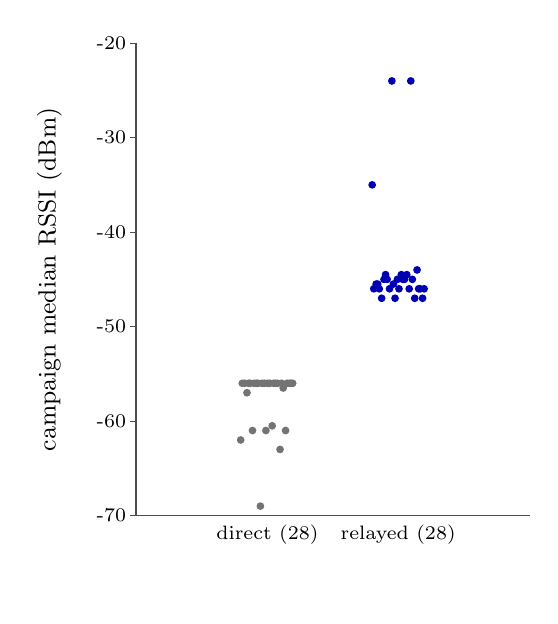
\begin{tikzpicture}[>=Latex, font=\footnotesize]
\draw[black!70] (0,0) -- (5,0);
\draw[black!70] (0,0) -- (0,6);
\draw[black!70] (0,0) -- ++(-0.08,0);
\node[font=\scriptsize, left] at (0,0) {-70};
\draw[black!70] (0,1.2) -- ++(-0.08,0);
\node[font=\scriptsize, left] at (0,1.2) {-60};
\draw[black!70] (0,2.4) -- ++(-0.08,0);
\node[font=\scriptsize, left] at (0,2.4) {-50};
\draw[black!70] (0,3.6) -- ++(-0.08,0);
\node[font=\scriptsize, left] at (0,3.6) {-40};
\draw[black!70] (0,4.8) -- ++(-0.08,0);
\node[font=\scriptsize, left] at (0,4.8) {-30};
\draw[black!70] (0,6) -- ++(-0.08,0);
\node[font=\scriptsize, left] at (0,6) {-20};
\node[font=\small] at (2.5,-0.9) {};
\node[font=\small, rotate=90] at (-1.1,3) {campaign median RSSI (dBm)};
\fill[black!55] (1.33,0.96) circle (1.4pt);
\fill[black!55] (1.58,0.12) circle (1.4pt);
\fill[black!55] (1.83,0.84) circle (1.4pt);
\fill[black!55] (1.41,1.56) circle (1.4pt);
\fill[black!55] (1.65,1.08) circle (1.4pt);
\fill[black!55] (1.9,1.08) circle (1.4pt);
\fill[black!55] (1.48,1.08) circle (1.4pt);
\fill[black!55] (1.73,1.14) circle (1.4pt);
\fill[black!55] (1.97,1.68) circle (1.4pt);
\fill[black!55] (1.55,1.68) circle (1.4pt);
\fill[black!55] (1.8,1.68) circle (1.4pt);
\fill[black!55] (1.38,1.68) circle (1.4pt);
\fill[black!55] (1.63,1.68) circle (1.4pt);
\fill[black!55] (1.87,1.62) circle (1.4pt);
\fill[black!55] (1.45,1.68) circle (1.4pt);
\fill[black!55] (1.7,1.68) circle (1.4pt);
\fill[black!55] (1.95,1.68) circle (1.4pt);
\fill[black!55] (1.53,1.68) circle (1.4pt);
\fill[black!55] (1.77,1.68) circle (1.4pt);
\fill[black!55] (1.35,1.68) circle (1.4pt);
\fill[black!55] (1.6,1.68) circle (1.4pt);
\fill[black!55] (1.85,1.68) circle (1.4pt);
\fill[black!55] (1.43,1.68) circle (1.4pt);
\fill[black!55] (1.67,1.68) circle (1.4pt);
\fill[black!55] (1.92,1.68) circle (1.4pt);
\fill[black!55] (1.5,1.68) circle (1.4pt);
\fill[black!55] (1.75,1.68) circle (1.4pt);
\fill[black!55] (1.99,1.68) circle (1.4pt);
\fill[blue!70!black] (3,4.2) circle (1.4pt);
\fill[blue!70!black] (3.25,5.52) circle (1.4pt);
\fill[blue!70!black] (3.49,5.52) circle (1.4pt);
\fill[blue!70!black] (3.07,2.94) circle (1.4pt);
\fill[blue!70!black] (3.32,3) circle (1.4pt);
\fill[blue!70!black] (3.57,3.12) circle (1.4pt);
\fill[blue!70!black] (3.15,3) circle (1.4pt);
\fill[blue!70!black] (3.39,3) circle (1.4pt);
\fill[blue!70!black] (3.64,2.76) circle (1.4pt);
\fill[blue!70!black] (3.22,2.88) circle (1.4pt);
\fill[blue!70!black] (3.47,2.88) circle (1.4pt);
\fill[blue!70!black] (3.05,2.94) circle (1.4pt);
\fill[blue!70!black] (3.29,2.76) circle (1.4pt);
\fill[blue!70!black] (3.54,2.76) circle (1.4pt);
\fill[blue!70!black] (3.12,2.76) circle (1.4pt);
\fill[blue!70!black] (3.37,3.06) circle (1.4pt);
\fill[blue!70!black] (3.61,2.88) circle (1.4pt);
\fill[blue!70!black] (3.19,3) circle (1.4pt);
\fill[blue!70!black] (3.44,3.06) circle (1.4pt);
\fill[blue!70!black] (3.02,2.88) circle (1.4pt);
\fill[blue!70!black] (3.27,2.94) circle (1.4pt);
\fill[blue!70!black] (3.51,3) circle (1.4pt);
\fill[blue!70!black] (3.09,2.88) circle (1.4pt);
\fill[blue!70!black] (3.34,2.88) circle (1.4pt);
\fill[blue!70!black] (3.59,2.88) circle (1.4pt);
\fill[blue!70!black] (3.17,3.06) circle (1.4pt);
\fill[blue!70!black] (3.41,3) circle (1.4pt);
\fill[blue!70!black] (3.66,2.88) circle (1.4pt);
\node[font=\scriptsize] at (1.67,-0.24) {direct (28)};
\node[font=\scriptsize] at (3.33,-0.24) {relayed (28)};
\end{tikzpicture}

\caption{Campaign median RSSI of the direct and relayed configurations at 2.24\,m (M-19 family, 28 campaigns per side). The separation follows the device the verifier talks to: Relay~B is 12\,cm from the car, the key is 2.24\,m away.}
\label{fig:rssi}
\end{figure}

\subsection{Failures and transport}

Under unicast, where the relay uses MAC-level acknowledgements, no relayed round timed out at any layout. The broadcast relay, which has no acknowledgement and was run only at 0.52\,m, lost 11 of 150 rounds (7.3\,\%). The failure comes from frames lost without acknowledgement rather than from the distance, which supports H2. The broadcast layout cannot separate the two causes, so this is evidence for the transport, not a distance experiment.

\section{Discussion: Mitigations Against the Measured Data}
\label{sec:discussion}

\textbf{Distance bounding.} Distance bounding measures the time of a short, fast challenge--response, and derives a distance bound from it~\cite{b16,b27,b28}. A relay can only add time, so it can only raise the estimate. The protocol needs a clock that resolves the propagation time of the exchange, which is about one nanosecond for 30\,cm. The BLE stack on the CYD has a microsecond-level timer and a connection grid of 50\,ms, so this hardware cannot resolve the time a distance-bounding protocol needs. The measured overhead of about 280\,ms is about $3\times10^{8}$ times the propagation time over 30\,cm, so a bound that is tight enough to see the relay would detect it. The problem is that such a bound is only as good as the clock.

\textbf{Latency bounds.} A bound on the round trip, as in Section~\ref{sec:bound}, is practical with the verifier's existing timer. It separates the configurations on this stack with 0 honest rejections and about 2\,\% relayed acceptances, but it is not a complete defence. The relayed distribution has a tail that reaches about 107\,ms in some campaigns, and the honest distribution has a tail that reaches 150\,ms. The bound therefore moves the attacker's problem to phase management and to hardware: a relay that uses a shorter connection interval, or a faster link, would move its distribution below the bound. Our results cannot exclude that.

\textbf{The timeout is the relay's budget.} The sweep (Section~\ref{sec:sweep}) shows that the relay stops authenticating when the latency it adds exceeds the verifier's timeout minus the honest relayed round trip. With a 2\,s timeout, the relay tolerates about 1,650\,ms of added latency. A verifier that uses a shorter timeout forces the attacker to be faster, and a verifier that uses a longer one makes the relay easier. The timeout therefore sets the attacker's budget and should be chosen from the honest distribution, not from a convention. The bench cannot tell us the timeout of any real vehicle, so this result applies to the bench and to the mechanism, not to a product.

\textbf{UWB ranging.} UWB ranging resolves the propagation time, and CCC Digital Key Release 3.0 includes UWB ranging~\cite{b9}. The literature shows both sides: Singh \emph{et al.} proposed pulse reordering~\cite{b5}, and later work reduced the measured distance of the secure HRP ranging through ghost peaks and clock manipulation~\cite{b6,b7,b8}. The bench has no UWB hardware and does not test it, so the discussion is a comparison, not a result.

\textbf{RSSI and multi-factor detectors.} Our RSSI result shows that signal strength carries information about the device the verifier talks to, not about the relay. Detectors that combine RSSI with round-trip time and context~\cite{b22,b23} can work, but this study cannot evaluate them, because the layout confounds the signal.

\section{Threats to Validity}
\label{sec:threats}

\textbf{Internal validity.} The campaigns alternated between baseline and relayed and were not randomized, and the phase of each campaign follows from its start time. The random start offset (M-19) makes the phases of different campaigns independent, but not the rounds within a campaign. We reduced this with the campaign as the unit, but the number of campaigns per set, eight to ten, can detect only large differences: detecting 25\,ms between two relayed configurations would need about 73 campaigns per configuration at 80\,\% power, because the relayed campaign medians vary with a standard deviation of 54\,ms. Only the overhead and the latency-bound results are resolved at this size.

\textbf{External validity.} The key is an ESP32 emulator, not a smartphone. The phone's Bluetooth stack has its own latency and scheduling, so the numbers cannot be transferred to a phone key without a new measurement. The relay is a GATT-level forwarder without link-layer encryption; a relay at the link layer, as Khan describes~\cite{b4}, or a conformant CCC Digital Key implementation~\cite{b9} is not covered. The bench uses one PHY (1\,Mbit/s), one verifier timeout (2\,s), and distances up to 2.24\,m, so the results do not extend to longer ranges.

\textbf{Construct validity.} The distances are the layout, estimated by the operator and not measured with an instrument. RSSI is an auxiliary observation, not a distance measurement. The injected delay is applied to the challenge leg only, and its effect is an added time in the tunnel leg of the round.

\textbf{Conclusion validity.} The sample sizes are small in campaigns, and the intervals are bootstrap intervals over campaigns, so they describe the campaign-to-campaign variation of this bench. Holm's correction is applied to the campaign-level p-values of the three main sets. The logistic and mixed models were not fitted.

\section{Conclusion}
\label{sec:conclusion}

We built a bench of four CYD boards to measure how a BLE relay changes the authentication of a challenge--response, with a control without relay. A relay adds about 280\,ms to the round trip, which is far larger than the honest variation, and every unicast relayed round was answered within the verifier's timeout. The relay stops authenticating when the latency it adds exceeds the timeout minus the honest round trip, which places the attacker's budget at about 1,650\,ms on this bench. A latency bound of 160\,ms rejected no honest round in 500 on a replication set and accepted 2.6\,\% of relayed rounds, so a timing bound narrows the attack but does not remove it. RSSI identified the device the verifier talked to, not the relay. The contribution is the protocol, the dataset and the characterization of the latency budget. The next steps are a measurement on a smartphone key, a layout that equalizes the relay and key distances for the RSSI test, and an attenuated tunnel for the distance limit.

\section*{Data and Code Availability}

The firmware, the analysis scripts, the raw logs with their manifests, the plans committed before the held-out and replication campaigns, and this paper's source are in the public repository \url{https://github.com/ricardomdcj/cybersec-pkes-relay}, under the MIT licence.

\begin{thebibliography}{00}
\bibitem{b1} A.~Francillon, B.~Danev, and S.~\v{C}apkun, ``Relay attacks on passive keyless entry and start systems in modern cars,'' in \emph{Proc. Netw. Distrib. Syst. Secur. Symp. (NDSS)}, San Diego, CA, USA, 2011.
\bibitem{b2} T.~Bianchi, A.~Brighente, M.~Conti, and E.~Pavan, ``SoK: Stealing cars since remote keyless entry introduction and how to defend from it,'' in \emph{Proc. USENIX Symp. Veh. Secur. Privacy (VehicleSec)}, 2025, pp.~161--178.
\bibitem{b3} P.~Staat, K.~Jansen, C.~Zenger, H.~Elders-Boll, and C.~Paar, ``Analog physical-layer relay attacks with application to Bluetooth and phase-based ranging,'' in \emph{Proc. 15th ACM Conf. Secur. Privacy Wireless Mobile Netw. (WiSec)}, 2022, pp.~60--72.
\bibitem{b4} S.~Q.~Khan, ``Technical advisory: Tesla BLE phone-as-a-key passive entry vulnerable to relay attacks,'' NCC Group, Manchester, U.K., May 15, 2022.
\bibitem{b5} M.~Singh, P.~Leu, and S.~\v{C}apkun, ``UWB with pulse reordering: Securing ranging against relay and physical-layer attacks,'' in \emph{Proc. Netw. Distrib. Syst. Secur. Symp. (NDSS)}, 2019.
\bibitem{b6} M.~Singh, M.~Roeschlin, E.~Zalzala, P.~Leu, and S.~\v{C}apkun, ``Security analysis of IEEE 802.15.4z/HRP UWB time-of-flight distance measurement,'' in \emph{Proc. 14th ACM Conf. Secur. Privacy Wireless Mobile Netw. (WiSec)}, 2021, pp.~227--237.
\bibitem{b7} P.~Leu, G.~Camurati, A.~Heinrich, M.~Roeschlin, C.~Anliker, M.~Hollick, S.~\v{C}apkun, and J.~Classen, ``Ghost peak: Practical distance reduction attacks against HRP UWB ranging,'' in \emph{Proc. 31st USENIX Secur. Symp.}, 2022, pp.~1343--1359.
\bibitem{b8} C.~Anliker, G.~Camurati, and S.~\v{C}apkun, ``Time for change: How clocks break UWB secure ranging,'' in \emph{Proc. 32nd USENIX Secur. Symp.}, 2023, pp.~19--36.
\bibitem{b9} Car Connectivity Consortium, ``Digital key release 3.0,'' Whitepaper, 2022.
\bibitem{b10} D.~Suresh, P.~V.~Joshi, and P.~Parandkar, ``Mitigating relay attacks in vehicle access systems using BLE and UWB,'' \emph{Eng. Technol. Appl. Sci. Res. (ETASR)}, vol.~15, no.~5, pp.~26965--26970, 2025.
\bibitem{b16} S.~Drimer and S.~J.~Murdoch, ``Keep your enemies close: Distance bounding against smartcard relay attacks,'' in \emph{Proc. 16th USENIX Secur. Symp.}, Boston, MA, USA, 2007, pp.~87--102.
\bibitem{b22} J.~Wang, K.~Lounis, and M.~Zulkernine, ``CSKES: A context-based secure keyless entry system,'' in \emph{Proc. IEEE Annu. Comput. Softw. Appl. Conf. (COMPSAC)}, 2019.
\bibitem{b23} G.~Revadigar, C.~Javali, and S.~K.~Jha, ``ProxiCar: Proximity-based secure digital key solution for cars,'' in \emph{Proc. Int. Conf. Commun. Syst. Netw. (COMSNETS)}, 2020.
\bibitem{b24} A.~Abidin, M.~El~Soussi, J.~Romme, P.~Boer, D.~Singel\'ee, and C.~Bachmann, ``Secure, accurate, and practical narrow-band ranging system,'' \emph{IACR Trans. Cryptogr. Hardw. Embed. Syst.}, vol.~2021, no.~2, pp.~106--135, 2021.
\bibitem{b25} X.~Xie, K.~Jiang, R.~Dai, J.~Lu, L.~Wang, Q.~Li, and J.~Yu, ``Access your Tesla without your awareness: Compromising keyless entry system of Model 3,'' in \emph{Proc. Netw. Distrib. Syst. Secur. Symp. (NDSS)}, 2023.
\bibitem{b26} D.~Suresh, P.~V.~Joshi, P.~Parandkar, A.~Gambhir, and K.~M.~Sudharshan, ``BLE channel sounding: Novel method for enhanced ranging accuracy in vehicle access,'' \emph{IEEE Access}, vol.~13, pp.~67531--67547, 2025.
\bibitem{b27} S.~Brands and D.~Chaum, ``Distance-bounding protocols,'' in \emph{Advances in Cryptology---EUROCRYPT'93}, LNCS vol.~765, Springer, 1993, pp.~344--359. DOI: 10.1007/3-540-48285-7\_30.
\bibitem{b28} G.~P.~Hancke and M.~G.~Kuhn, ``An RFID distance bounding protocol,'' in \emph{Proc. IEEE/Create-Net SecureComm}, Athens, Greece, 2005, pp.~67--73. DOI: 10.1109/SECURECOMM.2005.56.
\bibitem{b29} Espressif Systems, \emph{ESP32 Series Datasheet}, v5.3, Tables 5-6 to 5-8 (Wi-Fi and Bluetooth radio characteristics).
\bibitem{b30} IEEE Std 802.15.4z-2020, Amendment to IEEE Std 802.15.4: enhanced ultra-wideband physical layers and ranging techniques, 2020.
\end{thebibliography}

\EOD

\end{document}
